
\noindent
\textbf{芸術科学 太郎}
\vspace{1mm} \\
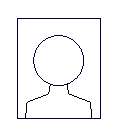
\includegraphics[width=25mm]{photo-face.eps} \\
1990年某大学理工学部電子通信学科卒業.
1992年某大学大学院理工学研究科電気工学専攻修士課程修了.
同年某社(株)入社.1997年博士(工学).
2000年米国某大学客員研究員.
2005年某社(株)退職,
2005年芸術科学大学大学院芸術科学研究科博士後期課程入学.
芸術と科学の接点に興味を持つ.
ACM, IEEE Computer Society, 芸術科学会,他会員.
%
\vspace{3mm}
\\
%
\textbf{芸術科学 次郎}
\vspace{1mm} \\
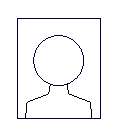
\includegraphics[width=25mm]{photo-face.eps} \\
1990年某大学理工学部電子通信学科卒業.
1992年某大学大学院理工学研究科電気工学専攻修士課程修了.
同年某社(株)入社.1997年博士(工学).
2000年米国某大学客員研究員.
2005年某社(株)退職,
2005年より芸術科学大学理学部情報科学科助教授,現在准教授.
芸術と科学の接点に興味を持つ.
ACM, IEEE Computer Society, 芸術科学会,他会員.
% ----

